\documentclass[12pt,letterpaper]{article}
    \usepackage[utf8]{inputenc}
    \usepackage{ifpdf}
    \makeatletter
    \@namedef{ver@thumbpdf.sty}{}
    \makeatother
    \usepackage{mla}
    \usepackage[pass]{geometry}
    \usepackage{todonotes}
    \usepackage{graphicx}
    \usepackage[hidelinks]{hyperref}
	\usepackage{float}
	\usepackage{soul}
	\usepackage{setspace}
    \urlstyle{same}

\begin{document}
\begin{mla}{Bernardo}{Meurer}{Professor Eckford-Prossor}{English 111 H}{April 30, 2018}{Essay 4 --- 321's\footnote{\st{I do not like this 321 at all. I think I wrote a bunch of crap. I'm sorry. At least the typesetting is good.}}\footnote{Actually now that I'm halfway through I like it more. Typesetting still good.}}
	%%% Quotes %%%
	\subsection*{3 --- Quotations}
	\begin{itemize}
		\item ``O you who turn the wheel and look to windward,\\ Consider Phlebas, who was once handsome and tall as you.''\\
		      --- I think there's this interesting dimension of ``cautionary tale'' that this passage clearly brings. This entire part of the poem, IV, is cryptic to me. I think in a way it brings forth how our qualities, being handsome and tall like Phlebas, may not save us from failure.

		\item ``Oed' und leer das Meer.'' --- ``Desolate and empty is the sea.''\\
		      ``I Tiresias, though blind, throbbing between two lives,\\
		      Old man with wrinkled female breasts, can see\\
		      At the violet hour, the evening hour that strives\\
		      Homeward, and brings the sailor home from sea,''\\
		      --- For some reason when I read this I was immediately reminded of the famous Portuguese short-story \textit{The Tale of the Unknown Island} by José Saramago, which you, Professor, should read as soon as possible. In the tale, the man who wanted a boat says ``O mar é sempre tenebroso,'' in the English edition this was translated as ``The sea is always obscure,'' which is fair, but not good. \textit{Tenebroso} means dark, scary, mysterious, unknown, afflicting, and complex (to comprehend.) Overall, it's an extremely dense word, and ``obscure'' doesn't quite capture it. In any sense, I just feel like this quote shows in a way a complete disconnect of Eliot's era, and our own, to the previous perception of the sea, as \textit{tenebroso.} In a rough transition, I just think the WWI era is this fascinating clash of old and new, and this, albeit maybe remotely, speaks to this.
		\item ``There I saw one I knew, and stopped him, crying “Stetson!\\
		      You who were with me in the ships at Mylae!\\
		      That corpse you planted last year in your garden,\\
		      Has it begun to sprout? Will it bloom this year?\\
		      Or has the sudden frost disturbed its bed?''\\
		      --- I just absolutely love this passage, it's such a good characterization of insanity. It's nonsensical, and yet it speaks deeply to the time-context of the poem, in particular to the absolute bizarre dimension of the first world war, and its impacts.

		\item \textbf{BONUS:} I thought you would enjoy this little poem by Nabokov, written on a letter to Edmund Wilson:
		      \begin{blocks}
			      At first my brain was somewhat numbed\\
			      by your somnambulistic numbers, Edmund.\\
			      Now, having shaken off that stupor,\\
			      I find the latter anagrimes with ``Proust''\\
			      while ``T.S. Eliot''\\
			      goes well with ``toilets.''\\
		      \end{blocks}
	\end{itemize}
	%%% Questions %%%
	\subsection*{2 --- Questions}
	\begin{itemize}
		\item How do the old and the new interface in the context of The Waste Land?\\ --- This comes from thoughts regarding the dychotomic nature of WWI, with it's sword-and-shield strategies but gunpowder weapons, for example. In an overarching sense how do these drastically disparate realities, being brought together by a quickly changing world/reality interface?
		\item In the 20th, and even more so in the 21st, century, is there space or chance for anything to be \textit{tenebroso} still? When everything is known by someone, and our existence is bound by laws and theorems, is there space for ``enchantment?''
	\end{itemize}
	%%% Essay %%%
	\subsection*{1 --- Essay}
	\paragraph*{The Age of Nothing}  \hspace{0pt} \\
	I took a train this weekend, from Santa Barbara down to Los Angeles and, despite Amtrak's striking punctuality, I found myself enjoying the trip. The railroad is quite scenic, until it goes into Oxnard, and then a number of farms start appearing out of nowhere, with irrigation so plentiful one would never judge California to be on a drought. In one of these fields there were a few dozen workers picking something that I made out to be tomatoes, but considering my sight could be anything, one by one. Here it struck me, some of those workers could have been working there for over a decade, in some sense farming, and yet I wondered whether they had ever touched the soil they step on. Even more so, I wondered whether whomever owns the farm ever touched on the soil they reap from; has anyone who works there? I wonder when was the last time one of them grabbed the soil to check for how moist it is, if any of them ever tasted the soil to check of it's too alkaline; I doubt it.

	In that farm, of course, the workers only reap what they have not sown; a machine planted the seeds after all. Seeds which, most likely, came from some lab, carefully engineered to grow into sterile plants. Fake seeds, planted by a machine, operated by someone who knows only the gauges and knobs of it, picked by man who know only how to pick, eaten by people who get it, cleaned, sterilized, pulverized, from a box; where did the farmer go? He's gone, of course; not fast enough, not productive enough, not scalable. Somehow along the way we seem to have lost a fundamental connection with ourselves; we seem to have forgotten that what we do should be meaningful, if not to others than to ourselves.

	\begin{figure}[H]
		\centering
		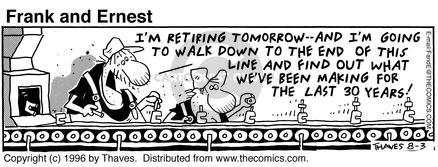
\includegraphics{assembly.jpg}
	\end{figure}
	Unfortunately, we haven't only lost ourselves in work, but this meaninglessness permeates modern life like a plague. People's social lives revolve around digital points, likes, loves, given to them by digital friends. We take pictures not to reminisce and long but to show our lives to mutually uninterested parties. We say vacuous words to endless pits of digital text wanting only to be heard. The message is secondary, what matters is that you have \textit{a} message, and everyone must know it, and see it, and like it, and share it. People talk endlessly on TV sets, YouTube, Facebook, and so many other platforms that will live and die like so many have; but what do they say?

	It is said that Flaubert wanted to write a romance about nothing, had he lived in our time he would've had great success.\footnote{Not to say Madame Bovary wasn't a great success.} We live in a conjecture so bizarre even out money is meaningless; what is a dollar after all? It's nothing, it's what people decide it to be worth. A dollar doesn't represent any physical quantity proper, not even the value of the paper that makes it; most of it is purely digital. Maybe I'm too simple-minded, but I find this existence to be overwhelming, somehow we have enslaved ourselves but we can't see it. I don't think Eliot could have predicted how deeply buried into nothing we would be, but he definitely shows us the roots of this trend.

	In ``I. The Burial of the Dead,'' of \textit{The Waste Land} Eliot writes:
	\begin{blocks}
		Unreal City,\hfill 60\\
		Under the brown fog of a winter dawn,\\
		A crowd flowed over London Bridge, so many,\\
		I had not thought death had undone so many.\\
		Sighs, short and infrequent, were exhaled,\\
		And each man fixed his eyes before his feet.\hfill 65\\
		Flowed up the hill and down King William Street,\\
		To where Saint Mary Woolnoth kept the hours\\
		With a dead sound on the final stroke of nine.\\
		\(\lbrack\ldots\rbrack \)
	\end{blocks}
	Where the ``crowd'' of undead refers to the huge numbers of proletariat-class workers marching towards their respective factories. Eliot's characterization of them as an undead crowd is extremely accurate, and is unchanged today. The same line could apply today, if only we replace ``feet'' for ``screen;'' feet are too gruesome after all. Again, somehow we've allowed death to undo as all, and endless crowd of undead men and women, of which I am a part of; how did we get here? Where has our sense of wonder and dazzle gone?

	For the last two hundred years or so we have lived in a post-enchantment world. Western society has been mostly disenchanted; in a world where everything is known by someone there is no need, or space, for magic or lore of any kind. It is because of this that religion, for example, has been on a slow but steady decline, allowing us to hear such pearls as ``I am morally Christian,'' which in non-euphemism means ``I don't believe in fairy tales, but I like the Christian moral-framework.'' How could they be Christian\footnote{This example uses Christianity for no particular reason. You can pick any religion, I believe.}, of course there is no God, there is only us; alone in our arrogance.

	Now, if there is no space for non-logic, and there is this overarching certainty that whatever it is that we may wonder about is already known by \emph{someone}, why wonder at all? Why should people waste their energy and time watching water go down the drain in a vortex and thinking ``Hmm, odd''? Worst even, for those that do consider it, why employ time into trying to conjecture a reason when Google knows it immediately? The answer to these questions may not be obvious, although it should, but it is simple: because it's what makes us Human\footnote{{Not sure whether to use ``Person'' or ``Human'' here. An acephalous new-born cannot reason, yet you wouldn't say they aren't Human, whilst you could argue they aren't a person.}}. What is the defining Human characteristic if not our ability, and our impulse, to reason. How else could we have gotten so far, so developed, so quickly if not by relentlessly questioning.

	It's no wonder Eliot calls us a crowd undone by death, we have lost that which makes us living humans. We've allowed others to convince us that things are too complex to be understood, we've allowed ourselves to delegate thinking to others, and reject our personhood; we must reclaim it. Let us allow the one who sows to reap as well, for the worker to ponder and reflect on his work. Let us allow ourselves to be fascinated by every day life, and to wonder, and err, about the reasons of things. Let us forget about the numerology in our memories, the shackles of the countably-invisible approval of others, and simply enjoy the moments we live in. We must allow ourselves to come back to life, and be human again.
	\newpage
	\paragraph*{Thoughts \& Questions}  \hspace{0pt} \\
	I like the essay, even though I think it's poorly written as it stands. I really like the title, could you give me some feedback on it? What do you think of the writing?

	I think the general point in question, that we've stopped wondering, is true, and a pet peeve of mine, but I find it hard to connect it more with the poem. Maybe relate it to the ``tamed'' drugged women? What do you think? Where else do you think this could tie in?

	Do I really need an op-ed? I don't like op-eds, and also I can't find something that ties in well with this, at least not how I'd like it to. I don't want to add a sausage-filling source that taints the paper in the end.

	Unlike Nabokov, I actually like the poem, it's nice. I'm writing more about my opinions on it in a ``class review'' I'm writing for you --- some (supposedly) useful feedback I've been accumulating throughout the semester.
\end{mla}
\end{document}
